\section{Background}

\subsection{Citation}
This is how you cite with both name and year surrounded by parentheses \parencite{anderson_chronic_2010}. 

This is how you manually specify the name and parentheses and cite with year (John Hopkins Medicine, \citeyear{john_hopkins_medicine_acute_2021}).

This is how you can cite multiple references within a pair of parentheses (not part of the citations) using square bracket (e.g., e.g., spinal cord injuries and disorders [John Hopkins Medicine, \citeyear{john_hopkins_medicine_acute_2021}; Meade, \citeyear{meade_health_2009}]).

This is how you cite multiple references \parencite{meade_health_2009, mamykina_mahi_2008,rooksby_personal_2014, murnane_personal_2018, raj_understanding_2017}.

This is how you can cite a reference with year in parentheses \textcite{anderson_patient_1995}.

\subsection{Styling}

\textcolor{\changecolor}{This is how you change the color of a segment of text.}

This is how you add a footnote \footnote{This is the actual footnote.}

This is how you create double quotes: ``double quotes.''

This is how you make text bold: \textbf{bold text}.


This is how you italicize text : \emph{italicized text} or \textit{another italicized text}.

This is how you create a link: \url{https://www.google.com/}.

This is how you create a list of bullet points:

\begin{itemize}
    \item A
    \item B
    \item C
\end{itemize}

This is how you create a quote block:

\begin{quote}
    I like this quote.
\end{quote}

\subsection{Table}

This is how you insert a table
\begin{table*}
    \caption{This is a table.}
    \label{tab:participant_table}
    \begin{tabular}{|p{0.7cm}|p{1.2cm}|p{1.5cm}|p{3.3cm}|p{4.3cm}|p{1.9cm}|}
      \toprule
       & Age & Gender & Background & Occupation & Experience\\
      \midrule
      P01 & 50-55 & F & Design & CEO & XYZ\\
      P02 & 50-55 & F & Design & CEO & XYZ\\
      \bottomrule
    \end{tabular}
  \end{table*}


\subsection{Figure}

This is how you insert a figure.
\begin{figure}[h]
    \centering
    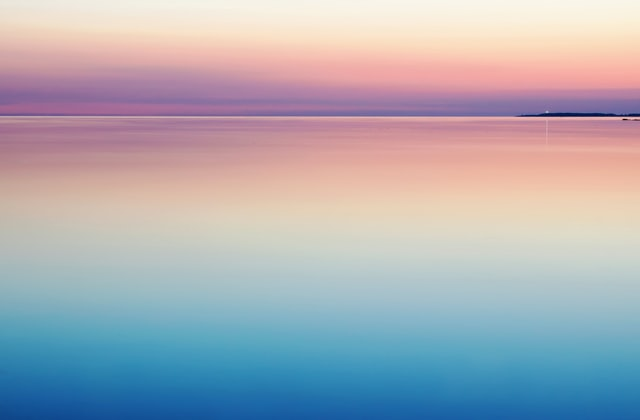
\includegraphics[width= \linewidth]{sources/introduction/images/harli-marten-n7a2OJDSZns-unsplash.jpg}
    \caption{Photo by Harli Marten on Unsplash}
    % https://unsplash.com/photos/n7a2OJDSZns
    \label{fig:my_figure_label}
  \end{figure}

\subsection{Referencing other materials}

In addition to tables and figures, you can use \label{my_label_name} for different sections.

This is how you can refer to another label: in Chapter~\ref{chap:3}.

This is how you can refer to a table: see Table ~\ref{tab:participant_table}.

This is how you can refer to a figure: in Figure~\ref{fig:my_figure_label}.



\subsection{Defining placeholders or variables}

You can use a command defined in definitions.tex as a placeholder in other tex files. The command will be replaced with \MyPlaceHolder{}.



\subsection{Additional Utilities}

In addition to standard Latex commenting using \%, you can use the following format to turn a big section of text into comment.

% content cut
\begin{comment}
A lot of comments here.
\end{comment}

You can add a to do inline:
\todo[inline]{Here is a inline todo item.}

You can also add a to do item directly:
\todo{Here is a todo item.}